\chapter{Implementation - Areas of Application}
\label{ch:impl_aoa}


\section{Manual editing (predefined structures)}
\label{sect:manual_editing}

	\begin{enumerate}
		\item \textbf{Build graph yourself}
		\item \textbf{Load predefined graph}
		\item \textbf{Watch visualization update}
		\item \textbf{run through whole algorithm at once (fluent vis??)}
	\end{enumerate}


\section{Graph extraction from images (graphs in preprocessing)}
\label{sect:graph_ext}

	\begin{enumerate}
		\item \textbf{Input image}
		\item \textbf{Image preprocessing}
		\item \textbf{graph based segmentation}
		\item \textbf{visualization}
	\end{enumerate}
	
	\begin{figure}[H]
		\begin{center}
			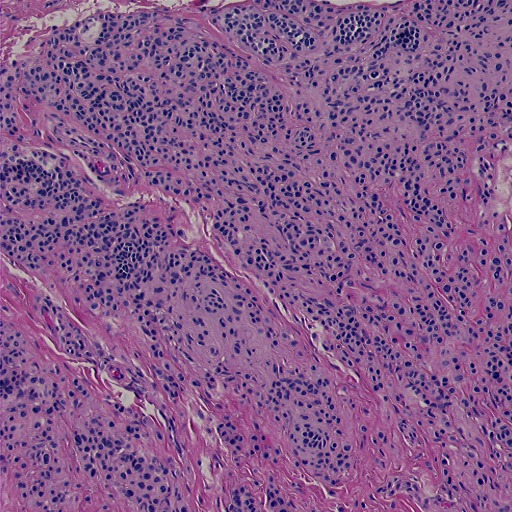
\includegraphics [width=0.24\textwidth] {figures/kruskal/sample2_input}
			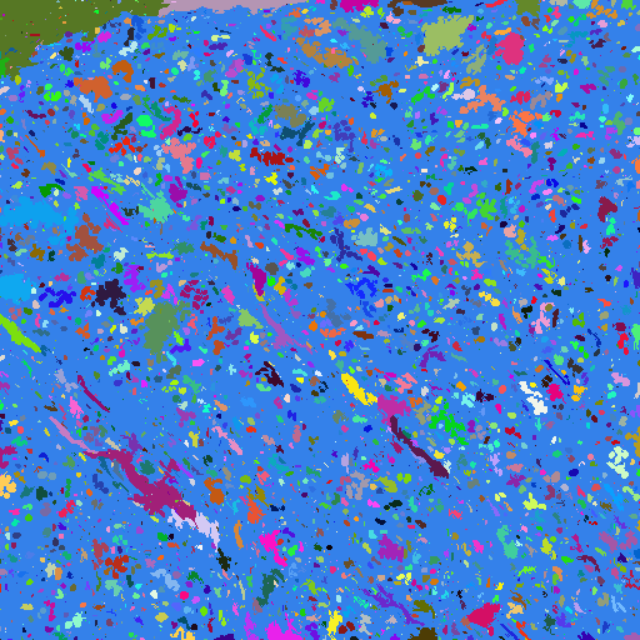
\includegraphics [width=0.24\textwidth] {figures/kruskal/out_rm_01}
			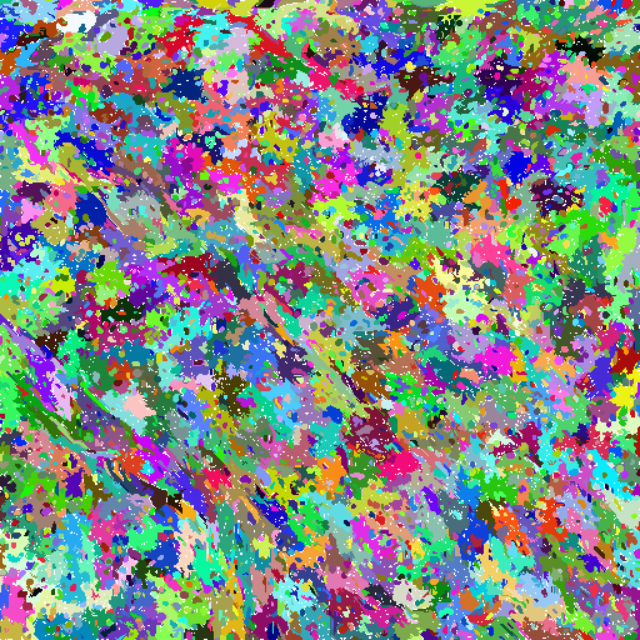
\includegraphics [width=0.24\textwidth] {figures/kruskal/out_rm_02}
			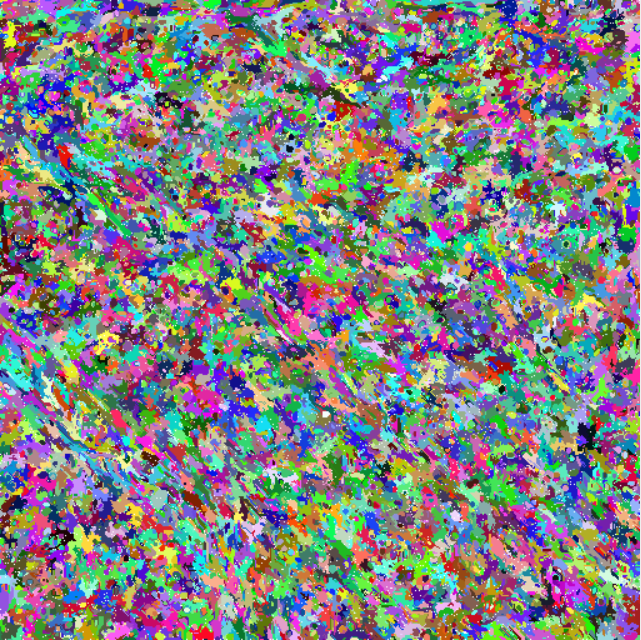
\includegraphics [width=0.24\textwidth] {figures/kruskal/out_rm_03}
			\caption{Kruskal MST based region merging}
		\end{center}
		\small 
		Result of applying a Kruskal based region merging algorithm to an image of numerous small scale regular structures. (1) Input image, (2) Result with parameters $k=1150, s=0, m=\infty$, (3) Result with parameters $k=150, s=5, m=500$, (4) Result with parameters $k=50, s=2, m=150 $.
		
	\end{figure}


\section{Anonymity: SaNGreeA (with iML)}
\label{sect:anonymization}

	\begin{enumerate}
		\item \textbf{Process input data into suitable structure}
		\item \textbf{Enhance structure with graph information (random)}
		\item \textbf{Anonymize via SaNGreeA}
		\item \textbf{prepare individual cost function via iML}
		\item \textbf{Anonymize via SaNGreeA modified}
		\item \textbf{Compare results}
	\end{enumerate}
	
	\begin{figure}[ht]
		\label{fig_anonIML}
		\begin{center}
			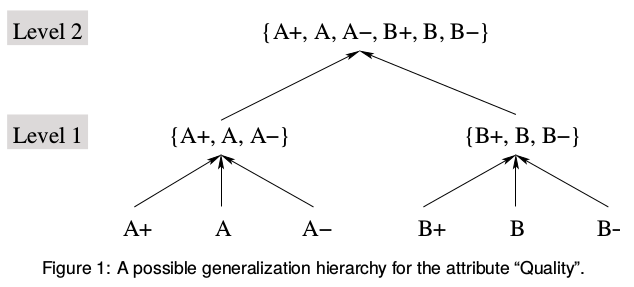
\includegraphics[width=0.8\textwidth]{figures/anonym/gen_hierarchy}
			\caption{Example of a typical generalization hierarchy}
		\end{center}
	\end{figure}	
	
	\begin{figure}[ht]
		\label{fig_anonIML}
		\begin{center}
			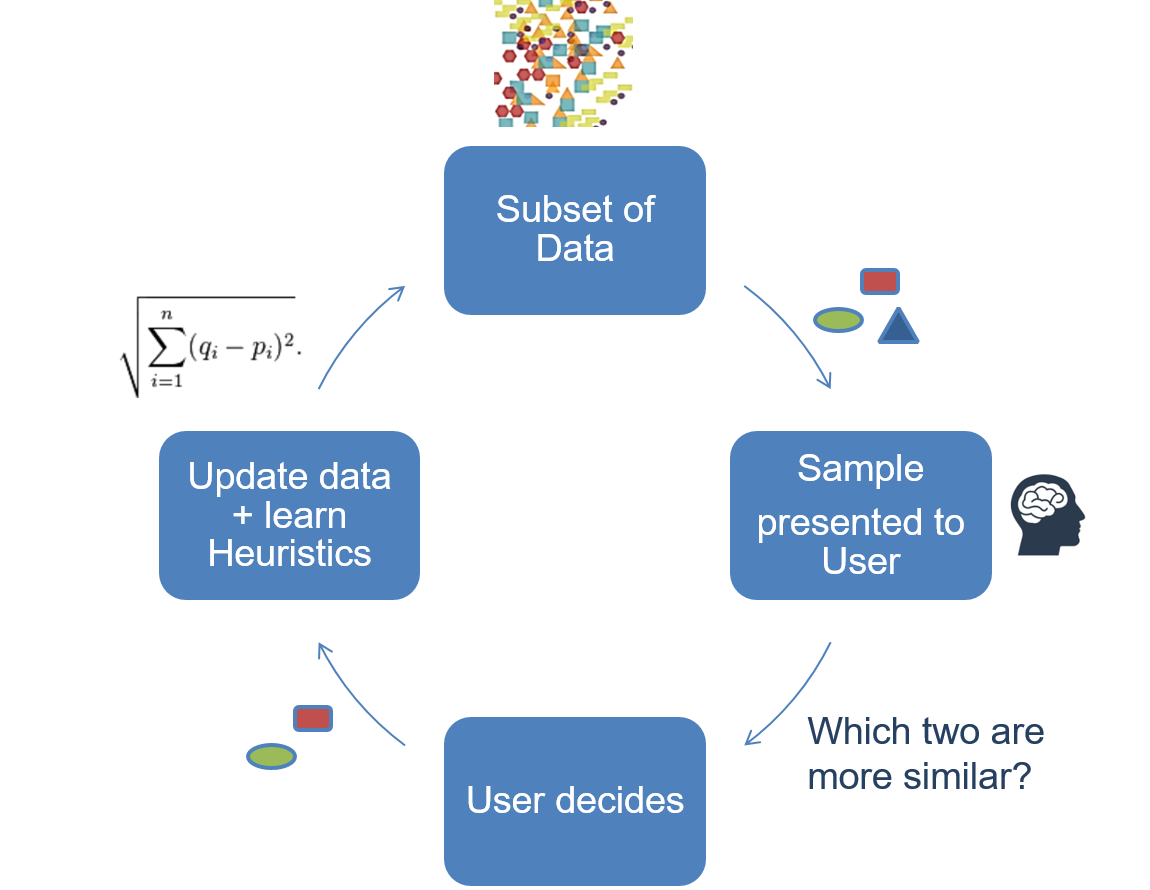
\includegraphics[width=1\textwidth]{figures/anonym/anonIML}
			\caption{Anonymization augmented by IML (human in the loop)}
		\end{center}
	\end{figure}


%\section{NLP: Community extraction \& group labeling (OPTIONAL !!)}
%\label{sect:nlp_community}
%
%	\begin{enumerate}
%		\item \textbf{Import and preprocess free text}
%		\item \textbf{Vectorize text in trigram feature space}
%		\item \textbf{Compute similarity kernel matrix}
%		\item \textbf{Extract connectivity graph from kernel matrix}
%		\item \textbf{Identify and extract communities from graph (SCC analysis?)} - node types
%		\item \textbf{Apply group labels to free text elements} - group labeling / node coloring
%	\end{enumerate}

